% =======================================================================================
\section{Flow Coordinates}
\label{app:chart}
% =======================================================================================

The flow does not transport physical parameters. A chart $\varphi$ maps each of the
$S=\ChartSources{}$ sources of a window to \ChartCoords{} real coordinates, so a window's sources
are a point of $\R^{\ChartCoords{}S}$, and the flow, its base distribution and its training paths
all live there. The chart depends on the window through its centre frequency $\fw$, so
converting between physical and flow coordinates always needs the $\fw$ of the observation.
\Cref{fig:chart} shows what the chart does to the prior.

\subsection{The Map}
\label{app:chart-map}

For a source with frequency $f_0$, chirp mass $\Mc$, amplitude $\Amp$, sky position
$(\alpha,\delta)$, polarisation angle $\psi$, inclination $\iota$ and initial phase $\phi_0$,
the chart is
\begin{equation}
\begin{aligned}
  x_f &= \frac{2\ln f_0 - \ln f_{\rm lo} - \ln f_{\rm hi}}{\ln f_{\rm hi} - \ln f_{\rm lo}}, &
  x_{\Mc} &= \frac{\ln\Mc - \mu_{\Mc}}{\sigma_{\Mc}}, &
  (x_l, x_b) &= \Bigl(\frac{l}{\sigma_l},\,\frac{b}{\sigma_b}\Bigr), \\
  z_\pm &= \operatorname{asinh}\lvert\zeta_\pm\rvert\,\frac{\zeta_\pm}{\lvert\zeta_\pm\rvert}, &
  \zeta_\pm &= \frac{\Amp}{u(\fw)}\,\frac{(1\mp\cos\iota)^2}{4}\,e^{\ii(\phi_0^{\rm mid}\pm2\psi)}, &
  u(f) &= \sqrt{S_n(f)/\Tobs},
\end{aligned}
\label{eq:chart}
\end{equation}
and the flow coordinates of the source are
$x = (x_f,\, x_{\Mc},\, x_l,\, x_b,\, \operatorname{Re}z_+,\, \operatorname{Im}z_+,\,
\operatorname{Re}z_-,\, \operatorname{Im}z_-)$, with $\phi_0^{\rm mid}$ the phase referred to
mid-observation (\cref{eq:chart-phase}). Each coordinate is shaped so that its prior has a scale
of order one and the chart has no singular or multiply covered point where the prior has mass.

\paragraph{Frequency.}
$[f_{\rm lo}, f_{\rm hi}]$ is the window interior of \cref{eq:priors-interior}, on which the
prior is log-uniform, so $x_f\sim\Unif(-1,1)$ exactly. One unit of $x_f$ spans $(4R-R)/2$ bins,
\ChartBinsPerUnitNarrow{} in the narrow band and \ChartBinsPerUnitFull{} in the full band. The flow
always predicts an order-one position inside the window; the absolute frequency reaches the
network through its conditioning on $\fw$ (\cref{app:network}). In single precision, $x_f$
resolves \num{\ChartFThirtyTwoBinsFull} bins near the window edges in the full band, far below
any posterior width.

\paragraph{Chirp mass.}
$\ln\Mc$ is standardised by its mean and standard deviation under the prior of
\cref{eq:priors-mc}, $e^{\mu_{\Mc}} = \qty{\ChartMcMedian}{\solarmass}$ and $\sigma_{\Mc} = \ChartMcLogStd{}$,
computed by quadrature.

\paragraph{Sky.}
The chart rotates $(\alpha,\delta)$ to galactic longitude and latitude, $l\in(-\pi,\pi]$ and
$b\in[-\pi/2,\pi/2]$, and divides each by its standard deviation under the sky prior
(\cref{eq:priors-sky}), $\sigma_l = \qty{\ChartSigmaL}{\radian}$ (\ang{\ChartSigmaLDeg}) and
$\sigma_b = \qty{\ChartSigmaB}{\radian}$ (\ang{\ChartSigmaBDeg}). The bulge and disks then sit at the
origin with unit scale. The chart's two defects lie where the prior is thinnest: the seam at the
anticentre, $l=\pm\pi$ ($x_l=\pm\ChartSeamX{}$), which holds \qty{\ChartSeamMass}{\percent} of the prior within
\ang{\ChartEdgeDeg}, and the galactic poles, $x_b=\pm\ChartPoleX{}$, which hold \qty{\ChartPoleMass}{\percent}
within \ang{\ChartEdgeDeg}. The inverse rotation maps any real $(l, b)$ to a direction, so the
flow's output never needs wrapping.

\paragraph{Helicity amplitudes.}
$\zeta_+$ and $\zeta_-$ are the complex amplitudes of the two circular polarisations in units
of $u(\fw)$, with $S_n$ the sky-averaged sensitivity of \cref{eq:noise-sky}
\citep[eq.~1]{robson2019construction} at the window centre, so that one unit holds across the
window. In these units the \ac{snr} of a source is $\snr = \kappa\,\Amp/u(\fw)$, and $\kappa$ is
set almost entirely by the inclination (\cref{fig:chart}c): averaged over the sky,
$\snr^2\propto\lvert\zeta_+\rvert^2+\lvert\zeta_-\rvert^2\propto 1+6\cos^2\iota+\cos^4\iota$, so
\begin{equation}
  \kappa^2 \approx C\,\frac{1+6\cos^2\iota+\cos^4\iota}{16/5},
  \label{eq:chart-kappa}
\end{equation}
where $16/5$ is the average of the numerator over $\cos\iota$ and $C = \ChartSkyConstant{}$ is the
mean of $\kappa^2$ over the galactic sky prior. The drawn sources follow \cref{eq:chart-kappa}
within \qty{\ChartKappaLawRms}{\percent} rms; $\kappa$ runs from \ChartKappaNarrowLow{} (edge-on) to
\ChartKappaNarrowHigh{} (face-on) in the narrow band and from \ChartKappaFullLow{} to
\ChartKappaFullHigh{} in the full band (1st and 99th percentiles), where the response departs from
its low-frequency limit. The radius is warped by $\operatorname{asinh}$, linear for faint
amplitudes and logarithmic for loud ones; at the top of the \ac{snr} range,
$\snr=\ChartSnrHigh{}$, it stays inside $\operatorname{asinh}\ChartSnrHigh{} = \ChartZReach{}$.

\begin{figure*}[t]
  \centering
  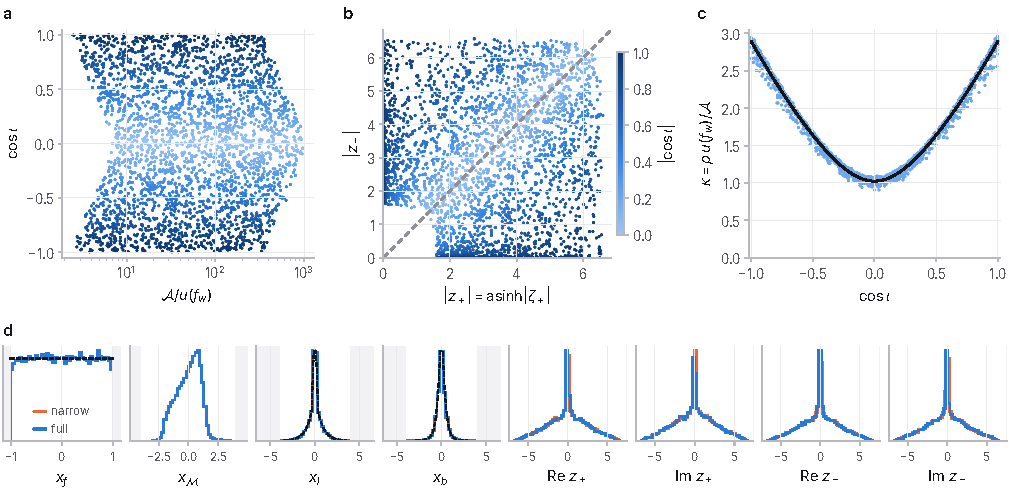
\includegraphics[width=\textwidth]{figures/chart.pdf}
  \caption{The helicity chart on prior draws. (a)~Amplitude in noise units against inclination
  for narrow-band sources; colour is $\lvert\cos\iota\rvert$ throughout (a,~b). The \ac{snr}
  range of the prior makes the amplitude range move with $\cos\iota$: the curved
  amplitude--inclination degeneracy is built into the prior. (b)~The same sources as the radii
  of the two helicity amplitudes. Face-on sources lie along the axes, with their weak helicity
  near zero; the \ac{snr} floor keeps the dominant helicity away from the origin. (c)~\ac{snr}
  per unit amplitude against inclination, with the sky-averaged law \cref{eq:chart-kappa}.
  (d)~The prior's marginal in each of the \ChartCoords{} flow coordinates, for both bands, with the
  closed-form marginal dashed where it exists. Shading marks coordinates beyond the range of the
  network's input embedding. The spike at zero in $z_\pm$ is the weak helicity of near-face-on
  sources.}
  \label{fig:chart}
\end{figure*}

\subsection{Why Helicity Amplitudes}
\label{app:chart-helicity}

\paragraph{Linearity.}
At fixed $(f_0, \Mc, \alpha, \delta)$ the waveform (\cref{app:forward-model}) is a linear
combination of two fixed templates, one per circular polarisation, with complex coefficients
$\zeta_\pm$. The likelihood \cref{eq:loglik} is therefore Gaussian in
$(\operatorname{Re}\zeta_\pm, \operatorname{Im}\zeta_\pm)$: the structure the
$\mathcal F$-statistic maximises over \citep{jaranowski1998data}, written in the
circular-polarisation coordinates of \citet{whelan2014new}. The four extrinsic parameters
$(\Amp, \iota, \psi, \phi_0)$ enter the data only through these four real numbers.

\paragraph{Exact symmetries.}
The map $(\psi,\phi_0)\mapsto(\phi_0^{\rm mid}+2\psi,\ \phi_0^{\rm mid}-2\psi) \bmod 2\pi$ has a kernel
generated by $\psi\mapsto\psi+\pi$ and $(\psi,\phi_0)\mapsto(\psi+\pi/2,\ \phi_0+\pi)$: exactly
the four copies of \cref{eq:psi-phi-symmetry}. All four map to one chart point, so where the
posterior in $(\psi,\phi_0)$ has four equivalent modes, the posterior in the chart has one. This
matters for flow matching beyond economy: with the copies as separate modes, the conditional
mean velocity the network regresses on (\cref{app:fm}) averages over the four copies early in
the path, and the phase information is washed out.

\paragraph{Face-on sources.}
At $\cos\iota=\pm1$ the wave is circularly polarised and only $\phi_0\pm2\psi$ is observable.
In the chart this is the point where one of $z_\pm$ vanishes, a regular point of the plane, not
a coordinate pole: a polar chart in $(\Amp, \cos\iota, \phi_0^{\rm mid}\pm2\psi)$ would have an
undefined phase there. Since $\operatorname{asinh}(r)/r$ is an even analytic function of $r$,
the warp $\zeta\mapsto\operatorname{asinh}\lvert\zeta\rvert\,\zeta/\lvert\zeta\rvert$ is a
diffeomorphism of $\mathbb C$, the origin included, with inverse
$z\mapsto\sinh\lvert z\rvert\,z/\lvert z\rvert$. The prior has much of its mass there
(\cref{fig:chart}b,d).

\paragraph{Amplitude and inclination.}
Away from edge-on one helicity dominates,
$\lvert\zeta_-\rvert/\lvert\zeta_+\rvert = \bigl((1+\cos\iota)/(1-\cos\iota)\bigr)^2$, and the
data measure the dominant amplitude much better than the weak one. In $(\Amp,\cos\iota)$ this
gives the familiar curved degeneracy, a distant face-on source against a nearer inclined one
(\cref{fig:chart}a). In the chart the same posterior is a compact blob in the dominant helicity's
plane and a roughly isotropic blob around the origin in the weak one's, whose radius is set by
the noise: the chart straightens the banana by construction.

\paragraph{Phase reference.}
The phase enters the chart referred to mid-observation,
\begin{equation}
  \phi_0^{\rm mid} = \phi_0 - \pi f_0\Tobs - \tfrac{\pi}{4}\fdot\Tobs^2,
  \label{eq:chart-phase}
\end{equation}
with $\fdot$ the chirp of $(f_0, \Mc)$ (\cref{app:forward-model}). The signal phase is
$-\phi_0 + 2\pi f_0 t + \pi\fdot t^2$, so $-\phi_0^{\rm mid}$ is the carrier phase at
$t=\Tobs/2$, the time centroid of a monochromatic signal, which the data fix independently of
$f_0$. Referred to $t=0$ instead, an error of $\delta$ bins in $f_0$ moves the phase by
$\pi\delta$~\unit{\radian}, which couples phase and frequency across the whole posterior. For each
$(f_0, \Mc)$, \cref{eq:chart-phase} is a rotation of the circle, so $\phi_0^{\rm mid}$ is
uniform and independent of the other parameters under the prior, as $\phi_0$ is.

\subsection{The Inverse Map}
\label{app:chart-inverse}

The frequency, chirp mass and sky invert directly. For the helicity amplitudes, with
$r_\pm = \sqrt{\sinh\lvert z_\pm\rvert}$,
\begin{equation}
  \sqrt{\Amp/u(\fw)} = r_+ + r_-, \qquad
  \cos\iota = \frac{r_- - r_+}{r_+ + r_-}, \qquad
  \psi = \tfrac14\bigl(\arg z_+ - \arg z_-\bigr), \qquad
  \phi_0^{\rm mid} = \tfrac12\bigl(\arg z_+ + \arg z_-\bigr),
  \label{eq:chart-inverse}
\end{equation}
since $\sqrt{\lvert\zeta_+\rvert}+\sqrt{\lvert\zeta_-\rvert}=\sqrt{\Amp/u}$ for every $\iota$.
\Cref{eq:chart-inverse} returns one of the four copies of \cref{eq:psi-phi-symmetry}, all
equivalent. The inverse is defined everywhere except at $\Amp=0$, where both $z_\pm$ vanish and
the orientation is undefined, a set of measure zero that the \ac{snr} floor of the prior
excludes.

\subsection{Flat Chart and Straight Paths}
\label{app:chart-flat}

All \ChartCoords{} coordinates are flat: the flow acts on $\R^{\ChartCoords{}}$ per source, with
no manifold, no angle with a branch cut and no exponential or logarithm map. The flow-matching
path between a base point $x_0$ and a target $x_1$ is the straight line
$x_s = x_0 + s\,(x_1 - x_0)$ of constant velocity $x_1 - x_0$ (\cref{app:fm}), and the sampler's
steps stay in the chart whatever the network predicts. The base distribution is the prior pushed
through \cref{eq:chart}, sampled by drawing physical parameters and mapping them, so neither
training nor sampling evaluates a density and the chart's Jacobian never enters.

The pushed-forward prior is not simple, but it is well scaled (\cref{fig:chart}d): $x_f$ is
uniform, the chirp mass and sky coordinates have standard deviations between
\ChartUnitStdLow{} and \ChartUnitStdHigh{}, the helicity components between \ChartZStdLow{} and
\ChartZStdHigh{}, and no pair of the \ChartCoords{} coordinates is correlated by more than
$\lvert r\rvert = \ChartMaxCorr{}$ over \ChartPriorDraws{} prior sources per band. The sky prior's
tails are long: \qty{\ChartBeyondL}{\percent} of its $x_l$ and \qty{\ChartBeyondB}{\percent} of its $x_b$ lie beyond
$\pm\ChartReach{}$, where the network's input embedding ends (\cref{app:network}).

A flat chart of the sphere distorts lengths away from $b=0$, but the prior sits near the
galactic plane, where the distortion is small, and its two defects carry the masses quoted
above. A Riemannian flow on the product of the sphere and the phase torus would remove them at the cost of
geodesic paths and exponential maps.

\subsection{Ordered Sources}
\label{app:chart-slots}

The $S$ sources of a window are exchangeable under the prior and the likelihood
(\cref{app:priors-symmetries}). We break the permutation symmetry by ordering: each window's
sources are sorted by their drawn \ac{snr}, loudest first, and since the amplitude is set to
give exactly that \ac{snr} (\cref{eq:priors-amp}), the order of the targets is exact. The base
draws are prior draws sorted the same way, so slot $i$ is transported from the $i$-th loudest
base draw to the $i$-th loudest source, with no alignment in the coupling, and each slot carries
a learned embedding of its rank (\cref{app:network}). Other amortised estimators for overlapping
sources order the sources in frequency \citep{delmond2026neural} or match per-source slots in
the loss by the Hungarian algorithm \citep{houba2025slotflow}; equivariant flow matching aligns
them instead \citep{klein2023equivariant}. An \ac{snr} ordering puts its boundary where two
sources are equally loud rather than where they are close in frequency.

The data do not fix the \ac{snr} exactly, so two sources of similar \ac{snr} can swap slots
between posterior draws. Scores against the injections therefore pair drawn slots with injected
sources by the cheapest assignment over frequency, amplitude and sky, and the calibration tests
relabel the truth and every draw by the same truth-independent rule, each draw's own \ac{snr},
loudest first (\cref{app:evaluation}).
